%!TEX root=seke.tex
% mainfile: ../seke.tex

% Box and whisker plots
% Belongs to results_bwplots, but must be here for positioning reasons

\begin{figure*}[t!]
\centering
\begin{subfigure}{0.5\textwidth}
  \centering
  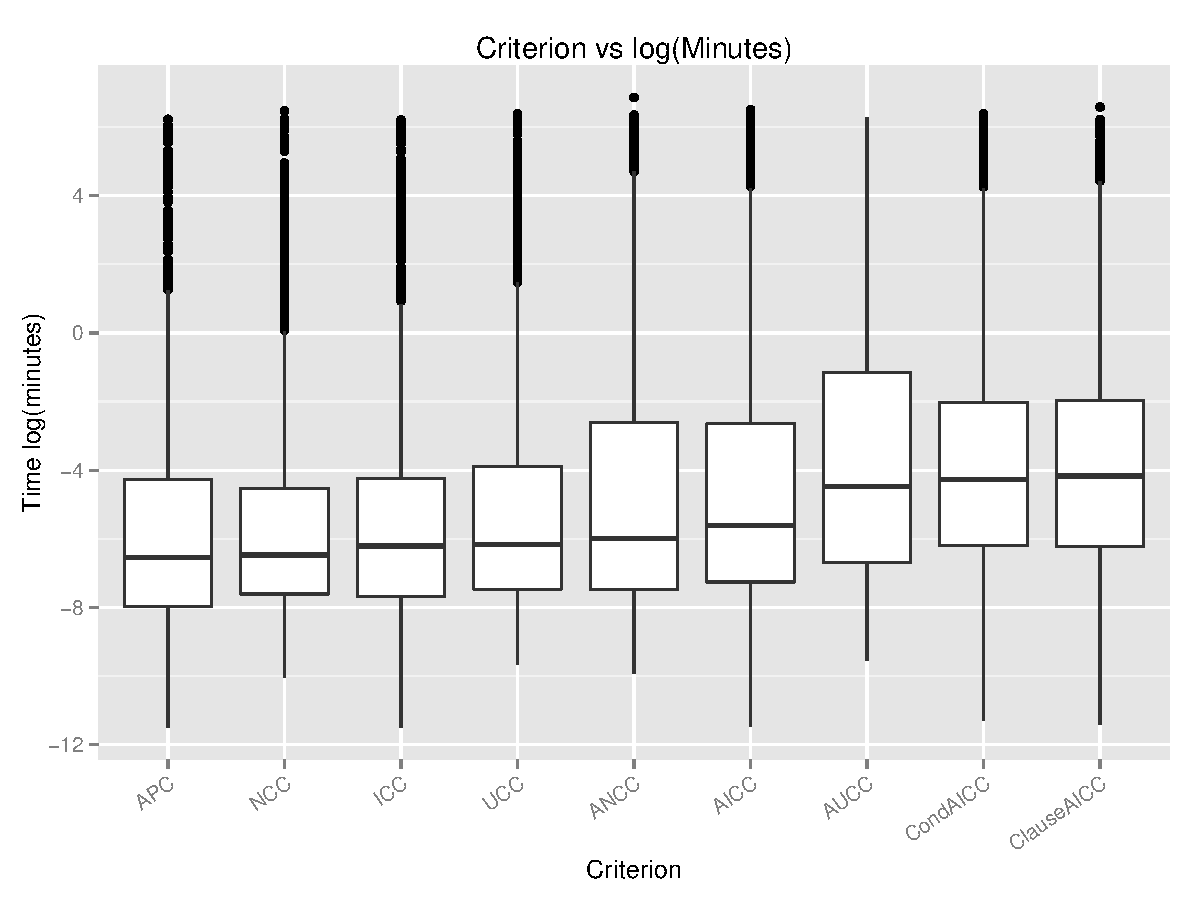
\includegraphics[width=1\linewidth]{diagrams/CriterionOrder.pdf}
  \caption{Coverage criterion versus runtime in minutes.}
  \label{fig:crites}
\end{subfigure}%
\begin{subfigure}{0.5\textwidth}
  \centering
  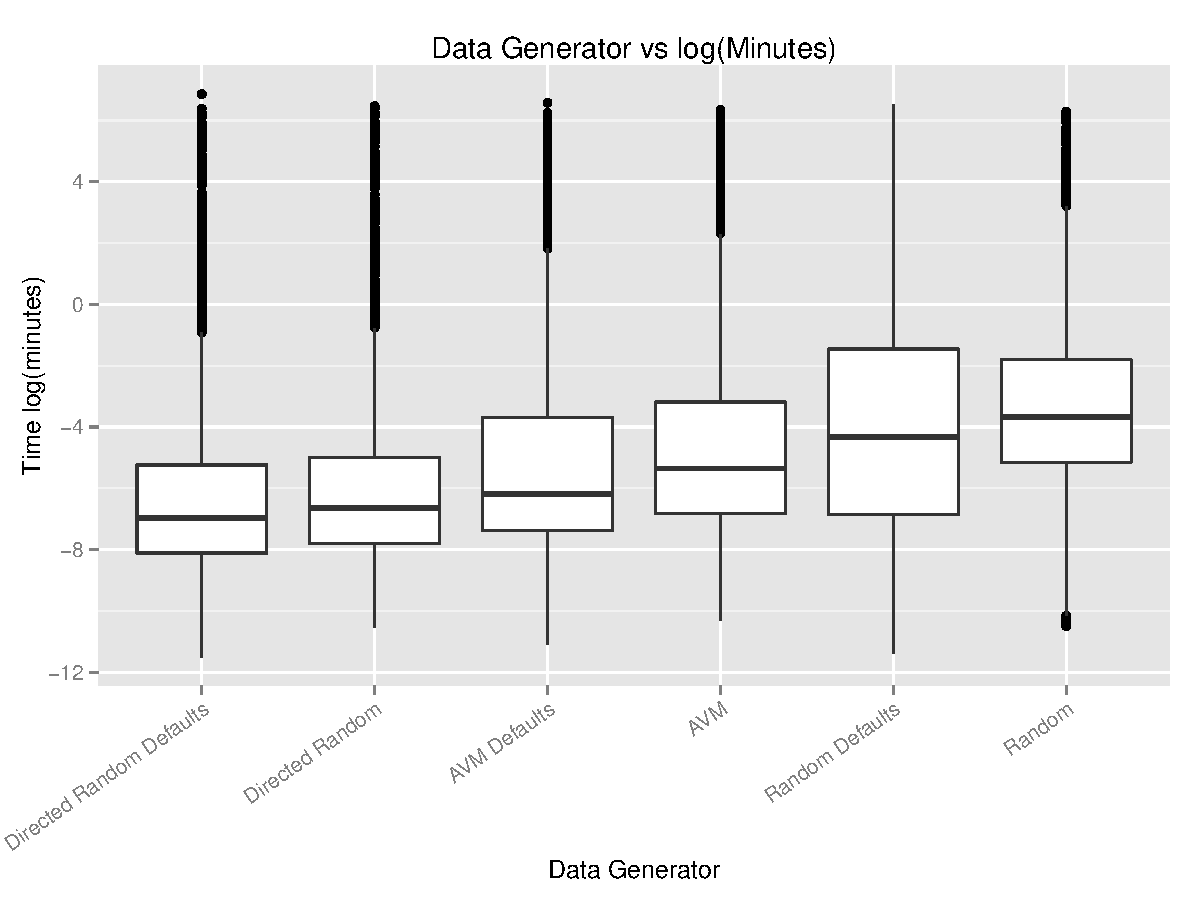
\includegraphics[width=1\linewidth]{diagrams/DataGeneratorOrder.pdf}
  \caption{Data generator versus runtime in minutes.}
  \label{fig:datas}
\end{subfigure}
\label{fig:bwplots}
\caption{Box and whisker plots for criterion and data
  generator.}
\end{figure*}

\textbf{Results}. Our experiments reveal that for the number of \texttt{UNIQUE}s, {\tt NOT NULL}s, and {\tt CHECK}s,
\textit{SchemaAnalyst} displays linear or linearithmic worst-case time complexity.  Out of the 699 experiments performed
doubling these schema structures, $72\%$ converged to linear or linearithmic.  Another $8\%$ failed to converge, and of
these experiments, $80\%$ failed because of memory limitations, $13\%$ exceeded the maximum time limit, and for $8\%$
the reason for failure could not be determined.  The doubling ratios among these experiments were primarily linear or
linerarithmic at the time they were terminated, however there were some that were quadratic and three that were cubic.
The experiments that failed to converge were primarily complicated schemas such as iTrust and BioSQL, and criteria at
the top of the hierarchy, such as ANCC and AUCC. The remaining $20\%$ converged on constant or logarithmic.  Since there
did not seem to be a pattern in which configurations converged this way compared to linear or linearithmic, it is
likely that these experiments terminated before the true worst-case time complexity was apparent.

For the schema structures tables and columns, the results were less conclusive. Doubling the number of tables in the
schema caused the runtime of \textit{SchemaAnalyst} to increase much faster than the integrity constraints. As a result,
$56\%$ of the 467 experiments doubling this schema feature were terminated after exceeding the experiment time limit
before they converged.  Of the experiments that converged, 72 converged to quadratic, and 10 converged to cubic.  Of the
experiments that terminated before they converged, the doubling ratios for 205 indicated quadratic, 18 indicated cubic,
and 37 were worse than cubic.

Experiments on the number of columns were also inconclusive.  208 experiments that converged showed linear or
linearithmic time complexity, while 28 converged to quadratic and 2 cubic.  Another 203 experiments failed to converge,
however unlike the experiments for the number of tables, the experiments for the number of columns most frequently
failed by running out of memory rather than running out of time. The experiments that did not converge include 106
ratios indicating quadratic behavior, 73 cubic, and 3 worse.

